\documentclass[tikz,border=8pt]{standalone}
\usepackage{amsmath}
\usetikzlibrary{arrows.meta}
\definecolor{latticeblue}{RGB}{27,102,170}
\definecolor{basisred}{RGB}{190,55,55}
\newcommand{\panel}[7]{%
  \begin{scope}[shift={(#1,#2)}]
    \node[font=\bfseries] at (0,2.35) {#3};
    \node[font=\scriptsize,align=center] at (0,-2.35) {#7};
    \clip (-2.35,-2.05) rectangle (2.35,2.05);
    \draw[gray!35,very thin] (-2.35,0)--(2.35,0) (0,-2.05)--(0,2.05);
    \foreach \m in {-5,...,5}{
      \foreach \n in {-5,...,5}{
        \fill[latticeblue] ({#6*(\m+\n*#4)},{#6*\n*#5}) circle (1.45pt);
      }
    }
    \draw[-{Stealth[length=4pt]},basisred,very thick] (0,0)--({#6},0);
    \draw[-{Stealth[length=4pt]},basisred,very thick] (0,0)--({#6*#4},{#6*#5});
  \end{scope}%
}
\begin{document}
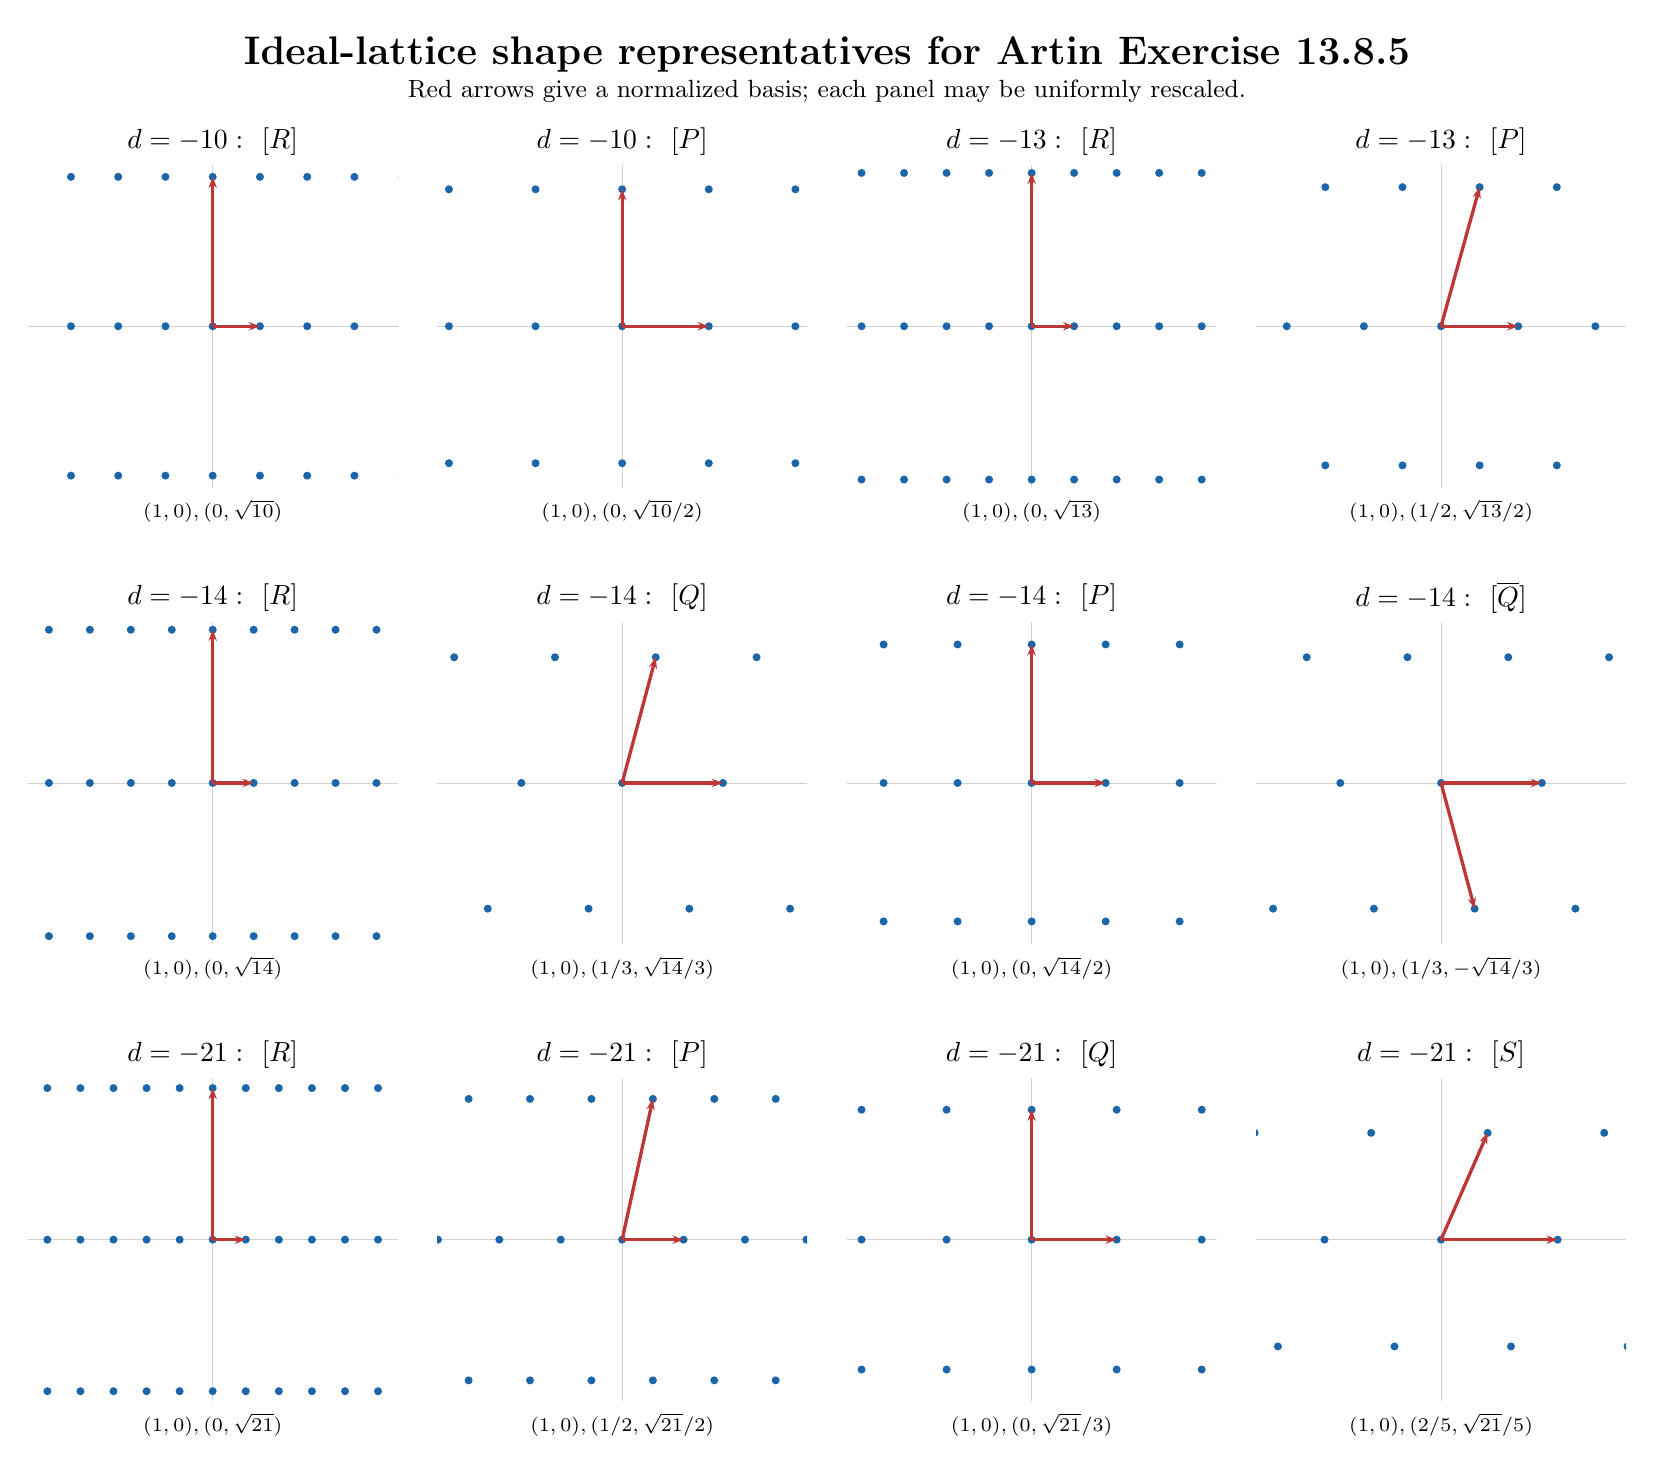
\begin{tikzpicture}[x=1cm,y=1cm]
  \node[font=\Large\bfseries] at (7.8,10.15) {Ideal-lattice shape representatives for Artin Exercise 13.8.5};
  \node[font=\small] at (7.8,9.68) {Red arrows give a normalized basis; each panel may be uniformly rescaled.};

  \panel{0}{6.7}{\(d=-10:\ [R]\)}{0}{3.1623}{0.60}{\((1,0),(0,\sqrt{10})\)}
  \panel{5.2}{6.7}{\(d=-10:\ [P]\)}{0}{1.5811}{1.10}{\((1,0),(0,\sqrt{10}/2)\)}
  \panel{10.4}{6.7}{\(d=-13:\ [R]\)}{0}{3.6056}{0.54}{\((1,0),(0,\sqrt{13})\)}
  \panel{15.6}{6.7}{\(d=-13:\ [P]\)}{0.5}{1.8028}{0.98}{\((1,0),(1/2,\sqrt{13}/2)\)}

  \panel{0}{0.9}{\(d=-14:\ [R]\)}{0}{3.7417}{0.52}{\((1,0),(0,\sqrt{14})\)}
  \panel{5.2}{0.9}{\(d=-14:\ [Q]\)}{0.3333}{1.2472}{1.28}{\((1,0),(1/3,\sqrt{14}/3)\)}
  \panel{10.4}{0.9}{\(d=-14:\ [P]\)}{0}{1.8708}{0.94}{\((1,0),(0,\sqrt{14}/2)\)}
  \panel{15.6}{0.9}{\(d=-14:\ [\overline Q]\)}{0.3333}{-1.2472}{1.28}{\((1,0),(1/3,-\sqrt{14}/3)\)}

  \panel{0}{-4.9}{\(d=-21:\ [R]\)}{0}{4.5826}{0.42}{\((1,0),(0,\sqrt{21})\)}
  \panel{5.2}{-4.9}{\(d=-21:\ [P]\)}{0.5}{2.2913}{0.78}{\((1,0),(1/2,\sqrt{21}/2)\)}
  \panel{10.4}{-4.9}{\(d=-21:\ [Q]\)}{0}{1.5275}{1.08}{\((1,0),(0,\sqrt{21}/3)\)}
  \panel{15.6}{-4.9}{\(d=-21:\ [S]\)}{0.4}{0.9165}{1.48}{\((1,0),(2/5,\sqrt{21}/5)\)}
\end{tikzpicture}
\end{document}
